% Options for packages loaded elsewhere
\PassOptionsToPackage{unicode}{hyperref}
\PassOptionsToPackage{hyphens}{url}
%
\documentclass[
]{article}
\usepackage{amsmath,amssymb}
\usepackage{iftex}
\ifPDFTeX
  \usepackage[T1]{fontenc}
  \usepackage[utf8]{inputenc}
  \usepackage{textcomp} % provide euro and other symbols
\else % if luatex or xetex
  \usepackage{unicode-math} % this also loads fontspec
  \defaultfontfeatures{Scale=MatchLowercase}
  \defaultfontfeatures[\rmfamily]{Ligatures=TeX,Scale=1}
\fi
\usepackage{lmodern}
\ifPDFTeX\else
  % xetex/luatex font selection
\fi
% Use upquote if available, for straight quotes in verbatim environments
\IfFileExists{upquote.sty}{\usepackage{upquote}}{}
\IfFileExists{microtype.sty}{% use microtype if available
  \usepackage[]{microtype}
  \UseMicrotypeSet[protrusion]{basicmath} % disable protrusion for tt fonts
}{}
\makeatletter
\@ifundefined{KOMAClassName}{% if non-KOMA class
  \IfFileExists{parskip.sty}{%
    \usepackage{parskip}
  }{% else
    \setlength{\parindent}{0pt}
    \setlength{\parskip}{6pt plus 2pt minus 1pt}}
}{% if KOMA class
  \KOMAoptions{parskip=half}}
\makeatother
\usepackage{xcolor}
\usepackage[margin=1in]{geometry}
\usepackage{color}
\usepackage{fancyvrb}
\newcommand{\VerbBar}{|}
\newcommand{\VERB}{\Verb[commandchars=\\\{\}]}
\DefineVerbatimEnvironment{Highlighting}{Verbatim}{commandchars=\\\{\}}
% Add ',fontsize=\small' for more characters per line
\usepackage{framed}
\definecolor{shadecolor}{RGB}{248,248,248}
\newenvironment{Shaded}{\begin{snugshade}}{\end{snugshade}}
\newcommand{\AlertTok}[1]{\textcolor[rgb]{0.94,0.16,0.16}{#1}}
\newcommand{\AnnotationTok}[1]{\textcolor[rgb]{0.56,0.35,0.01}{\textbf{\textit{#1}}}}
\newcommand{\AttributeTok}[1]{\textcolor[rgb]{0.13,0.29,0.53}{#1}}
\newcommand{\BaseNTok}[1]{\textcolor[rgb]{0.00,0.00,0.81}{#1}}
\newcommand{\BuiltInTok}[1]{#1}
\newcommand{\CharTok}[1]{\textcolor[rgb]{0.31,0.60,0.02}{#1}}
\newcommand{\CommentTok}[1]{\textcolor[rgb]{0.56,0.35,0.01}{\textit{#1}}}
\newcommand{\CommentVarTok}[1]{\textcolor[rgb]{0.56,0.35,0.01}{\textbf{\textit{#1}}}}
\newcommand{\ConstantTok}[1]{\textcolor[rgb]{0.56,0.35,0.01}{#1}}
\newcommand{\ControlFlowTok}[1]{\textcolor[rgb]{0.13,0.29,0.53}{\textbf{#1}}}
\newcommand{\DataTypeTok}[1]{\textcolor[rgb]{0.13,0.29,0.53}{#1}}
\newcommand{\DecValTok}[1]{\textcolor[rgb]{0.00,0.00,0.81}{#1}}
\newcommand{\DocumentationTok}[1]{\textcolor[rgb]{0.56,0.35,0.01}{\textbf{\textit{#1}}}}
\newcommand{\ErrorTok}[1]{\textcolor[rgb]{0.64,0.00,0.00}{\textbf{#1}}}
\newcommand{\ExtensionTok}[1]{#1}
\newcommand{\FloatTok}[1]{\textcolor[rgb]{0.00,0.00,0.81}{#1}}
\newcommand{\FunctionTok}[1]{\textcolor[rgb]{0.13,0.29,0.53}{\textbf{#1}}}
\newcommand{\ImportTok}[1]{#1}
\newcommand{\InformationTok}[1]{\textcolor[rgb]{0.56,0.35,0.01}{\textbf{\textit{#1}}}}
\newcommand{\KeywordTok}[1]{\textcolor[rgb]{0.13,0.29,0.53}{\textbf{#1}}}
\newcommand{\NormalTok}[1]{#1}
\newcommand{\OperatorTok}[1]{\textcolor[rgb]{0.81,0.36,0.00}{\textbf{#1}}}
\newcommand{\OtherTok}[1]{\textcolor[rgb]{0.56,0.35,0.01}{#1}}
\newcommand{\PreprocessorTok}[1]{\textcolor[rgb]{0.56,0.35,0.01}{\textit{#1}}}
\newcommand{\RegionMarkerTok}[1]{#1}
\newcommand{\SpecialCharTok}[1]{\textcolor[rgb]{0.81,0.36,0.00}{\textbf{#1}}}
\newcommand{\SpecialStringTok}[1]{\textcolor[rgb]{0.31,0.60,0.02}{#1}}
\newcommand{\StringTok}[1]{\textcolor[rgb]{0.31,0.60,0.02}{#1}}
\newcommand{\VariableTok}[1]{\textcolor[rgb]{0.00,0.00,0.00}{#1}}
\newcommand{\VerbatimStringTok}[1]{\textcolor[rgb]{0.31,0.60,0.02}{#1}}
\newcommand{\WarningTok}[1]{\textcolor[rgb]{0.56,0.35,0.01}{\textbf{\textit{#1}}}}
\usepackage{longtable,booktabs,array}
\usepackage{calc} % for calculating minipage widths
% Correct order of tables after \paragraph or \subparagraph
\usepackage{etoolbox}
\makeatletter
\patchcmd\longtable{\par}{\if@noskipsec\mbox{}\fi\par}{}{}
\makeatother
% Allow footnotes in longtable head/foot
\IfFileExists{footnotehyper.sty}{\usepackage{footnotehyper}}{\usepackage{footnote}}
\makesavenoteenv{longtable}
\usepackage{graphicx}
\makeatletter
\def\maxwidth{\ifdim\Gin@nat@width>\linewidth\linewidth\else\Gin@nat@width\fi}
\def\maxheight{\ifdim\Gin@nat@height>\textheight\textheight\else\Gin@nat@height\fi}
\makeatother
% Scale images if necessary, so that they will not overflow the page
% margins by default, and it is still possible to overwrite the defaults
% using explicit options in \includegraphics[width, height, ...]{}
\setkeys{Gin}{width=\maxwidth,height=\maxheight,keepaspectratio}
% Set default figure placement to htbp
\makeatletter
\def\fps@figure{htbp}
\makeatother
\setlength{\emergencystretch}{3em} % prevent overfull lines
\providecommand{\tightlist}{%
  \setlength{\itemsep}{0pt}\setlength{\parskip}{0pt}}
\setcounter{secnumdepth}{-\maxdimen} % remove section numbering
\usepackage{booktabs}
\usepackage{longtable}
\usepackage{array}
\usepackage{multirow}
\usepackage{wrapfig}
\usepackage{float}
\usepackage{colortbl}
\usepackage{pdflscape}
\usepackage{tabu}
\usepackage{threeparttable}
\usepackage{threeparttablex}
\usepackage[normalem]{ulem}
\usepackage{makecell}
\usepackage{xcolor}
\ifLuaTeX
  \usepackage{selnolig}  % disable illegal ligatures
\fi
\IfFileExists{bookmark.sty}{\usepackage{bookmark}}{\usepackage{hyperref}}
\IfFileExists{xurl.sty}{\usepackage{xurl}}{} % add URL line breaks if available
\urlstyle{same}
\hypersetup{
  pdftitle={Kaufman\_McNeill\_ENV797\_Project},
  pdfauthor={Emma Kaufman and Jenn McNeill},
  hidelinks,
  pdfcreator={LaTeX via pandoc}}

\title{Kaufman\_McNeill\_ENV797\_Project}
\author{Emma Kaufman and Jenn McNeill}
\date{2024-04-10}

\begin{document}
\maketitle

\begin{Shaded}
\begin{Highlighting}[]
\CommentTok{\# load required packages}
\FunctionTok{library}\NormalTok{(lubridate)}
\end{Highlighting}
\end{Shaded}

\begin{verbatim}
## 
## Attaching package: 'lubridate'
\end{verbatim}

\begin{verbatim}
## The following objects are masked from 'package:base':
## 
##     date, intersect, setdiff, union
\end{verbatim}

\begin{Shaded}
\begin{Highlighting}[]
\FunctionTok{library}\NormalTok{(ggplot2)}
\FunctionTok{library}\NormalTok{(forecast)  }
\end{Highlighting}
\end{Shaded}

\begin{verbatim}
## Registered S3 method overwritten by 'quantmod':
##   method            from
##   as.zoo.data.frame zoo
\end{verbatim}

\begin{Shaded}
\begin{Highlighting}[]
\FunctionTok{library}\NormalTok{(Kendall)}
\FunctionTok{library}\NormalTok{(tseries)}
\FunctionTok{library}\NormalTok{(outliers)}
\FunctionTok{library}\NormalTok{(tidyverse)}
\end{Highlighting}
\end{Shaded}

\begin{verbatim}
## -- Attaching core tidyverse packages ------------------------ tidyverse 2.0.0 --
## v dplyr   1.1.3     v stringr 1.5.0
## v forcats 1.0.0     v tibble  3.2.1
## v purrr   1.0.2     v tidyr   1.3.0
## v readr   2.1.4
\end{verbatim}

\begin{verbatim}
## -- Conflicts ------------------------------------------ tidyverse_conflicts() --
## x dplyr::filter() masks stats::filter()
## x dplyr::lag()    masks stats::lag()
## i Use the conflicted package (<http://conflicted.r-lib.org/>) to force all conflicts to become errors
\end{verbatim}

\begin{Shaded}
\begin{Highlighting}[]
\FunctionTok{library}\NormalTok{(smooth)}
\end{Highlighting}
\end{Shaded}

\begin{verbatim}
## Loading required package: greybox
## Package "greybox", v2.0.0 loaded.
## 
## 
## Attaching package: 'greybox'
## 
## The following object is masked from 'package:tidyr':
## 
##     spread
## 
## The following object is masked from 'package:lubridate':
## 
##     hm
## 
## This is package "smooth", v4.0.0
\end{verbatim}

\begin{Shaded}
\begin{Highlighting}[]
\FunctionTok{library}\NormalTok{(dplyr)}
\FunctionTok{library}\NormalTok{(cowplot)}
\end{Highlighting}
\end{Shaded}

\begin{verbatim}
## 
## Attaching package: 'cowplot'
## 
## The following object is masked from 'package:lubridate':
## 
##     stamp
\end{verbatim}

\begin{Shaded}
\begin{Highlighting}[]
\FunctionTok{library}\NormalTok{(corrplot)}
\end{Highlighting}
\end{Shaded}

\begin{verbatim}
## corrplot 0.92 loaded
\end{verbatim}

\begin{Shaded}
\begin{Highlighting}[]
\FunctionTok{library}\NormalTok{(kableExtra) }
\end{Highlighting}
\end{Shaded}

\begin{verbatim}
## 
## Attaching package: 'kableExtra'
## 
## The following object is masked from 'package:dplyr':
## 
##     group_rows
\end{verbatim}

\begin{Shaded}
\begin{Highlighting}[]
\FunctionTok{library}\NormalTok{(gridExtra)}
\end{Highlighting}
\end{Shaded}

\begin{verbatim}
## 
## Attaching package: 'gridExtra'
## 
## The following object is masked from 'package:dplyr':
## 
##     combine
\end{verbatim}

\hypertarget{introduction-motivation-relevance-objectives}{%
\paragraph{Introduction, Motivation, Relevance,
Objectives}\label{introduction-motivation-relevance-objectives}}

This project focuses on predicting water availability in an Italian
aquifer managed by Acea Group, a leading Italian utility operator. The
group provides water services to 9 million inhabitants across Italy.

In order to best service their customers, the Acea group must understand
how much water is available in the water bodies from which they extract.
Forecasting water availability in a water body is necessary to ensure
daily consumption needs are met.

The UN reported that groundwater provides ``half of the volume of water
withdrawn for domestic use by the global population'' and that water use
is expected to grow 1\% per year over the next thirty years (UN, 2022).
Thus, it is important to explore how much groundwater will be available
in the future. If groundwater levels are forecasted to drop
dramatically, these forecasts can be used to urge for more efficient
water use practices and investments into groundwater recharge
strategies.

We focused our study in Italy due to the comprehensive data we were able
to access in the region. In the following report, we examine the best
exogenous variables that can help accurately predict groundwater levels.
We hope that these findings offer insight about how to focus groundwater
forecasting efforts in other regions across the globe.

(add more about objectives?)

\hypertarget{dataset-information}{%
\paragraph{Dataset information}\label{dataset-information}}

Provide information on how the dataset for this analysis were collected
(source), the data contained in the dataset (format). Describe how you
wrangled/processed your dataset to get the time series object.

Add a table that summarizes your data structure (variables, units,
ranges and/or central tendencies, data source if multiple are used,
etc.). This table should inserted as a \texttt{kable} function in an R
chunk. Just show the first 10 rows of your data. Do not include the code
used to generate your table.

The dataset for this analysis was collected from the
\href{https://www.kaggle.com/c/acea-water-prediction/data}{Acea Group
Smart Water Analytics Competition on Kaggle}. As a utility operator,
they are concerned with preserving their water bodies which include a
combination of water springs, lakes, rivers, and aquifers. The nine
unique datasets from this kaggle competition each had different
attributes and characteristics. For our final project, we focused our
time series modeling and forecasting on the Auser Aquifer. Our objective
is to predict the amount of water in the Auser Aquifer by modeling the
depth to groundwater and simultaneously evaluating how rainfall and
temperature may impact our predictions as exogenous variables.

The dataset for the Auser Aquifer includes daily depth to groundwater
measurements (in meters) from five different wells across the north and
south sectors. Wells SAL, PAG, CoS, and DIEC represent the northern
unconfined portion while Well LT2 represents the southern confined
portion. We also have daily temperature data at four sites, daily
rainfall data at ten sites, and daily volume data from five different
water treatment facilities.

\begin{verbatim}
## [1] "/home/guest/TSA_Sp2024/Finalproj_EK_JM_TSA_Sp24"
\end{verbatim}

\begin{figure}
\centering
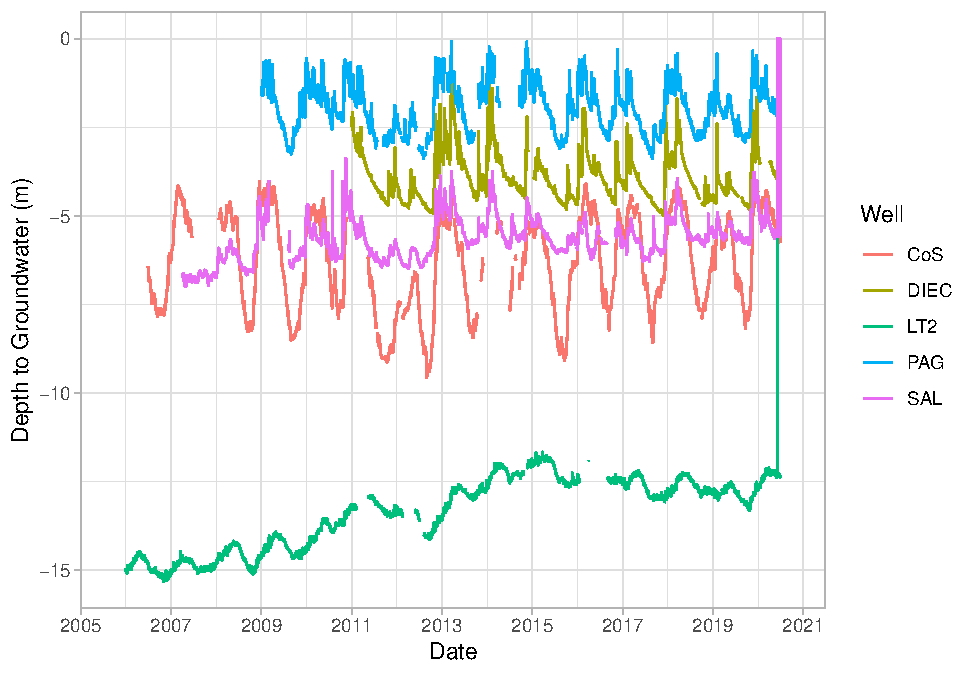
\includegraphics{Kaufman_McNeill_ENV797_Project_files/figure-latex/import data-1.pdf}
\caption{Raw}
\end{figure}

\begin{verbatim}
##  [1] -12.23 -12.22 -12.19 -12.25 -12.27 -12.27 -12.28 -12.25 -12.24 -12.28
## [11] -12.33 -12.33 -12.32 -12.34 -12.35 -12.38 -12.35 -12.33 -12.31 -12.31
## [21] -12.32 -12.30 -12.28 -12.22 -12.20   0.00   0.00 -12.27 -12.28 -12.28
## [31] -12.27 -12.29 -12.29 -12.27 -12.28 -12.28 -12.27 -12.29 -12.31 -12.32
## [41] -12.31 -12.33 -12.34 -12.35 -12.35 -12.36 -12.36 -12.37 -12.36 -12.38
\end{verbatim}

\begin{verbatim}
##  [1] -5.50 -5.47 -5.47 -5.43 -5.52 -5.53 -5.43 -5.47 -5.41 -5.42 -5.42 -5.46
## [13] -5.41 -5.51 -5.49 -5.42 -5.47 -5.52 -5.45 -5.43 -5.51 -5.48 -5.58 -5.55
## [25]  0.00  0.00  0.00 -5.30 -5.30 -5.27  0.00  0.00  0.00  0.00  0.00  0.00
## [37] -5.33 -5.34 -5.34 -5.29 -5.38 -5.43 -5.35 -5.46 -5.57  0.00 -5.50 -5.49
## [49] -5.50 -5.56
\end{verbatim}

\begin{verbatim}
##  [1] -1.87 -1.89 -1.93 -1.97 -2.00 -2.02 -2.06 -2.00 -1.71 -1.81 -1.89 -1.97
## [13] -2.02 -2.04 -2.06 -2.11 -2.09 -2.06 -2.07 -2.14 -2.15 -2.17 -2.21 -2.11
## [25] -2.10 -2.14 -2.14 -2.12 -2.12 -2.02 -2.01 -2.07 -2.07 -1.82 -1.88 -1.94
## [37] -1.54 -1.37 -1.57 -1.70 -1.78 -1.85 -1.92 -1.97 -2.03 -2.04 -2.10 -2.14
## [49] -2.15 -2.17
\end{verbatim}

\begin{verbatim}
##  [1] -5.13 -5.16 -5.13 -5.17 -5.21 -5.28 -5.31 -5.24 -5.19 -5.22 -5.29 -5.37
## [13] -5.42 -5.41 -5.43 -5.47 -5.54 -5.47 -5.46 -5.54 -5.53 -5.58 -5.63 -5.60
## [25]  0.00  0.00  0.00 -5.75 -5.78 -5.74 -5.63 -5.60 -5.63 -5.59 -5.51 -5.50
## [37] -5.45 -5.37 -5.33 -5.37 -5.39 -5.39 -5.44 -5.51 -5.59  0.00 -5.71 -5.73
## [49] -5.73 -5.76
\end{verbatim}

\begin{verbatim}
##  [1] -3.75 -3.77 -3.80 -3.83 -3.84 -3.85 -3.85 -3.86 -3.85 -3.87 -3.87 -3.88
## [13] -3.89 -3.90 -3.91 -3.93 -3.93 -3.92 -3.93 -3.94 -3.94 -3.95 -3.95 -3.88
## [25] -2.95 -3.13 -3.33 -3.38 -3.52 -3.60 -3.68 -3.75 -3.79 -3.79 -3.82 -3.83
## [37] -3.80 -3.75 -3.79 -3.80 -3.78 -3.79 -3.81 -3.82 -3.82 -3.83 -3.84 -3.84
## [49] -3.84 -3.85
\end{verbatim}

\begin{table}
\centering
\caption{\label{tab:data head and data variables kable}Auser Aquifer Data Head 10 Rows}
\centering
\fontsize{12}{14}\selectfont
\begin{tabular}[t]{l|l|l|l|l|l|l|l|l|l|l}
\hline
Date & 05-17-11 & 05-18-11 & 05-19-11 & 05-20-11 & 05-21-11 & 05-22-11 & 05-23-11 & 05-24-11 & 05-25-11 & 05-26-11\\
\hline
Rainfall\_Gallicano & 0.0 & 0.0 & 0.0 & 0.8 & 0.0 & 0.0 & 0.0 & 0.0 & 0.0 & 0.0\\
\hline
Rainfall\_Pontetetto & 0 & 0 & 0 & 0 & 0 & 0 & 0 & 0 & 0 & 0\\
\hline
Rainfall\_Monte\_Serra & 0 & 0 & 0 & 0 & 0 & 0 & 0 & 0 & 0 & 0\\
\hline
Rainfall\_Orentano & 0.0 & 0.0 & 0.0 & 0.2 & 0.0 & 0.0 & 0.0 & 0.0 & 0.0 & 0.0\\
\hline
Rainfall\_Borgo\_a\_Mozzano & 0 & 0 & 0 & 0 & 0 & 0 & 0 & 0 & 0 & 0\\
\hline
Rainfall\_Piaggione & 0 & 0 & 0 & 0 & 0 & 0 & 0 & 0 & 0 & 0\\
\hline
Rainfall\_Calavorno & 0 & 0 & 0 & 0 & 0 & 2 & 0 & 0 & 0 & 0\\
\hline
Rainfall\_Croce\_Arcana & 0.0 & 0.0 & 0.0 & 0.0 & 1.0 & 0.2 & 0.0 & 0.0 & 0.0 & 0.0\\
\hline
Rainfall\_Tereglio\_Coreglia\_Antelminelli & 0.0 & 0.0 & 0.0 & 0.6 & 0.0 & 0.0 & 0.0 & 0.0 & 0.0 & 0.0\\
\hline
Rainfall\_Fabbriche\_di\_Vallico & 0.0 & 0.0 & 0.0 & 0.4 & 0.0 & 0.0 & 0.0 & 0.0 & 0.0 & 0.0\\
\hline
Depth\_to\_Groundwater\_LT2 & -12.97 & -12.93 & -12.92 & -12.93 & -12.92 & -12.91 & -12.93 & -12.94 & -12.94 & -12.93\\
\hline
Depth\_to\_Groundwater\_SAL & -5.92 & -5.93 & -5.95 & -5.95 & -5.95 & -5.97 & -6.01 & -6.03 & -6.05 & -6.09\\
\hline
Depth\_to\_Groundwater\_PAG & -2.34 & -2.46 & -2.41 & -2.48 & -2.43 & -2.54 & -2.46 & -2.47 & -2.59 & -2.61\\
\hline
Depth\_to\_Groundwater\_CoS & -6.22 & -6.27 & -6.32 & -6.39 & -6.49 & -6.62 & -6.70 & -6.70 & -6.72 & -6.72\\
\hline
Depth\_to\_Groundwater\_DIEC & -3.79 & -3.80 & -3.80 & -3.81 & -3.81 & -3.82 & -3.83 & -3.84 & -3.84 & -3.85\\
\hline
Temperature\_Orentano & 16.05 & 17.20 & 19.25 & 20.65 & 20.40 & 21.65 & 22.15 & 24.35 & 23.30 & 23.85\\
\hline
Temperature\_Monte\_Serra & 12.80 & 15.25 & 15.35 & 16.40 & 17.60 & 18.65 & 20.25 & 20.20 & 21.30 & 20.25\\
\hline
Temperature\_Ponte\_a\_Moriano & 17.20 & 19.00 & 19.95 & 20.15 & 21.35 & 22.60 & 23.70 & 24.30 & 24.95 & 24.25\\
\hline
Temperature\_Lucca\_Orto\_Botanico & 17.45 & 19.00 & 20.10 & 21.60 & 21.15 & 22.55 & 23.60 & 24.05 & 24.60 & 24.70\\
\hline
Volume\_POL & -9936.0 & -9936.0 & -9936.0 & -9936.0 & -9936.0 & -9439.2 & -9936.0 & -9936.0 & -9936.0 & -9936.0\\
\hline
Volume\_CC1 & -16377.12 & -16377.12 & -16377.12 & -16377.12 & -16377.12 & -15558.26 & -16377.12 & -16377.12 & -16377.12 & -16377.12\\
\hline
Volume\_CC2 & -12823.49 & -12823.49 & -12823.49 & -12823.49 & -12823.49 & -12182.31 & -12823.49 & -12823.49 & -12823.49 & -12823.49\\
\hline
Volume\_CSA & 0 & 0 & 0 & 0 & 0 & 0 & 0 & 0 & 0 & 0\\
\hline
Volume\_CSAL & 0 & 0 & 0 & 0 & 0 & 0 & 0 & 0 & 0 & 0\\
\hline
Hydrometry\_Monte\_S\_Quirico & 0.17 & 0.18 & 0.16 & 0.15 & 0.15 & 0.15 & 0.15 & 0.14 & 0.15 & 0.14\\
\hline
Hydrometry\_Piaggione & -1.04 & -1.04 & -1.04 & -1.04 & -1.05 & -1.05 & -1.05 & -1.05 & -1.05 & -1.06\\
\hline
\end{tabular}
\end{table}

\begin{table}[!h]
\centering
\caption{\label{tab:data head and data variables kable}Acea Group Auser Aquifer Data Structure}
\centering
\fontsize{12}{14}\selectfont
\begin{tabular}[t]{l|l}
\hline
Variables & Units\\
\hline
Date & Date\\
\cline{1-2}
Rainfall\_Gallicano & \\
\cline{1-1}
Rainfall\_Pontetetto & \\
\cline{1-1}
Rainfall\_Monte\_Serra & \\
\cline{1-1}
Rainfall\_Orentano & \\
\cline{1-1}
Rainfall\_Borgo\_a\_Mozzano & \\
\cline{1-1}
Rainfall\_Piaggione & \\
\cline{1-1}
Rainfall\_Calavorno & \\
\cline{1-1}
Rainfall\_Croce\_Arcana & \\
\cline{1-1}
Rainfall\_Tereglio\_Coreglia\_Antelminelli & \\
\cline{1-1}
Rainfall\_Fabbriche\_di\_Vallico & \multirow[t]{-10}{*}{\raggedright\arraybackslash Millimeters}\\
\cline{1-2}
Depth\_to\_Groundwater\_LT2 & \\
\cline{1-1}
Depth\_to\_Groundwater\_SAL & \\
\cline{1-1}
Depth\_to\_Groundwater\_PAG & \\
\cline{1-1}
Depth\_to\_Groundwater\_CoS & \\
\cline{1-1}
Depth\_to\_Groundwater\_DIEC & \multirow[t]{-5}{*}{\raggedright\arraybackslash Meters}\\
\cline{1-2}
Temperature\_Orentano & \\
\cline{1-1}
Temperature\_Monte\_Serra & \\
\cline{1-1}
Temperature\_Ponte\_a\_Moriano & \\
\cline{1-1}
Temperature\_Lucca\_Orto\_Botanico & \multirow[t]{-4}{*}{\raggedright\arraybackslash Celcius}\\
\cline{1-2}
Volume\_POL & \\
\cline{1-1}
Volume\_CC1 & \\
\cline{1-1}
Volume\_CC2 & \\
\cline{1-1}
Volume\_CSA & \\
\cline{1-1}
Volume\_CSAL & \multirow[t]{-5}{*}{\raggedright\arraybackslash Cubic Meters}\\
\cline{1-2}
Hydrometry\_Monte\_S\_Quirico & \\
\cline{1-1}
Hydrometry\_Piaggione & \multirow[t]{-2}{*}{\raggedright\arraybackslash Meters}\\
\hline
\end{tabular}
\end{table}

The first obstacle with wrangling our data came when we realized that
the data for each variable started at a different date. We found this
issue by plotting the five depth to groundwater lines and seeing a large
lag before the data started, NA values within each series, and a few
random ``zero'' values that we assumed to be errors. To rectify this
issue, we converted all ``zero'' values to NA, found the start date for
each well's data, and then converted each well's data into a time series
object. When we plotted these five time series together, we still had
gaps of NA data. We ran the tsclean() function to fill in the gaps of
missing data with interpolated values and then had five clean series
with no data gaps.

\begin{verbatim}
## Scale for x is already present.
## Adding another scale for x, which will replace the existing scale.
\end{verbatim}

\begin{figure}
\centering
\includegraphics{Kaufman_McNeill_ENV797_Project_files/figure-latex/clean time series-1.pdf}
\caption{Depth to Groundwater Time Series}
\end{figure}

\begin{verbatim}
## Scale for x is already present.
## Adding another scale for x, which will replace the existing scale.
\end{verbatim}

\begin{figure}
\centering
\includegraphics{Kaufman_McNeill_ENV797_Project_files/figure-latex/unnamed-chunk-2-1.pdf}
\caption{LT2 and SAL Time Series}
\end{figure}

\hypertarget{analysis-methods-and-models}{%
\paragraph{Analysis (Methods and
Models)}\label{analysis-methods-and-models}}

Describe the analysis and tests that were performed. Described the
components of the time series you identified. List any packages and
functions used. Include visualizations of your dataset (i.e.~time series
plot, ACF, PACF, etc).

Format your R chunks so that graphs are displayed but code is not
displayed. Accompany these graphs with text sections that describe the
visualizations and provide context for further analyses.

Each figure should be accompanied by a caption, and referenced within
the text if applicable.

The first step of analysis that we performed was running the correlation
function on our depth to groundwater data to discern whether the depth
to groundwater values at the five wells were correlated to one another.
We found that the four north wells had similar correlation values to one
another and that the one south well was weakly correlated to the others.
Because there were not strong correlations between the wells, we decided
to focus the rest of our analysis on one north, confined well (SAL) and
one south, unconfined well (LT2). These two wells had the most complete
time series data.

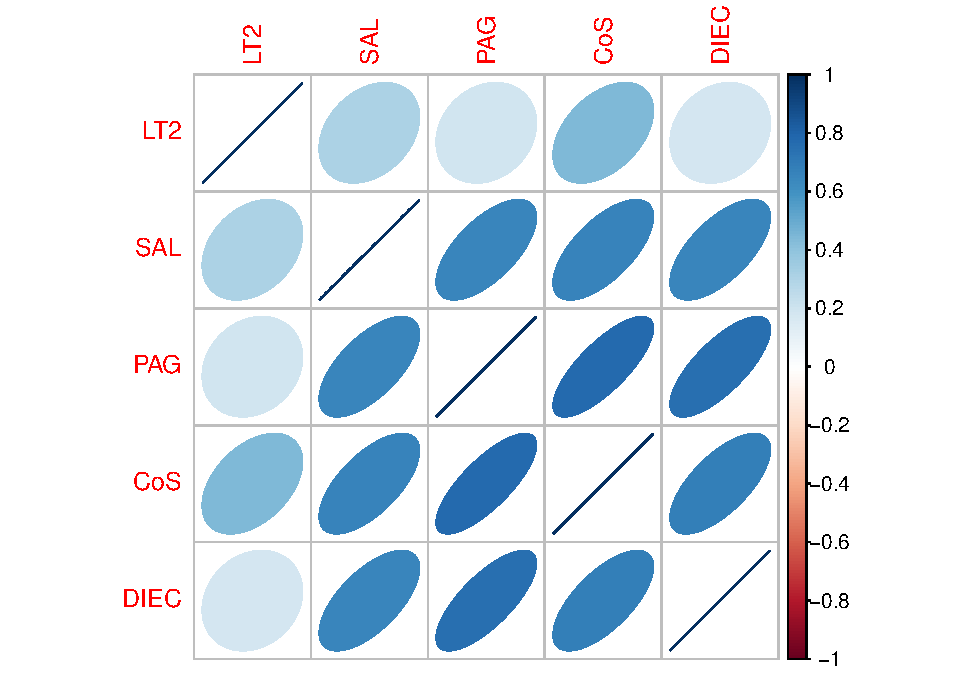
\includegraphics{Kaufman_McNeill_ENV797_Project_files/figure-latex/correlation plots-1.pdf}
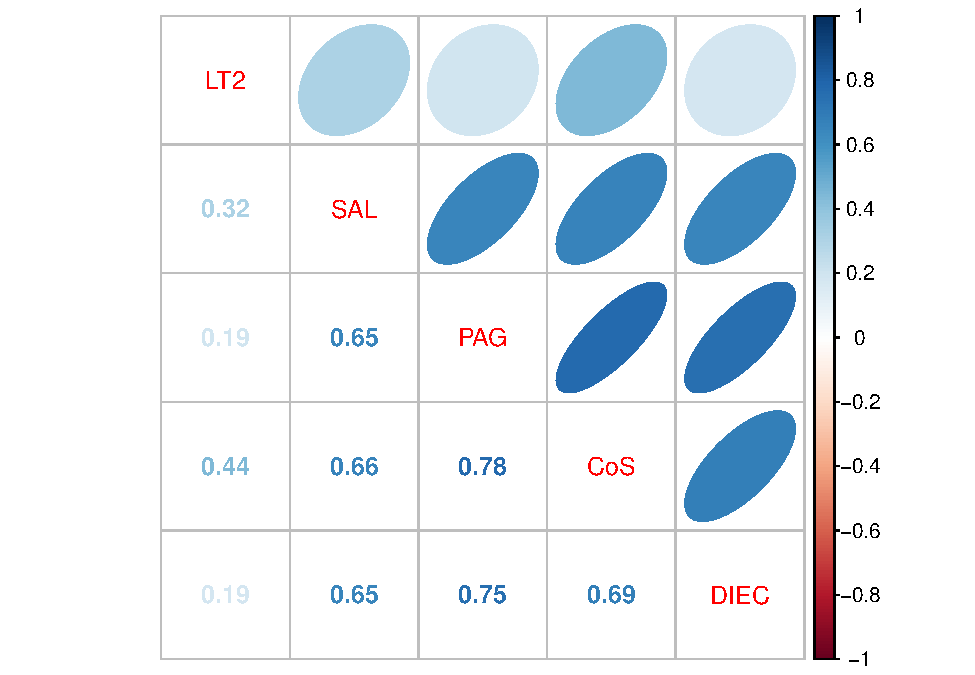
\includegraphics{Kaufman_McNeill_ENV797_Project_files/figure-latex/correlation plots-2.pdf}

We plotted the ACF and PACF for each well using a lag time of five years
to get a sense for whether our data had seasonal patterns. Both ACF
graphs show peaks and troughs at regular intervals, so we know that our
data has yearly seasonality. Knowing what we know about temperature and
rainfall affecting aquifer storage, it makes sense that the depth to
groundwater in the aquifer is changing with respect to the season.

\begin{figure}
\centering
\includegraphics{Kaufman_McNeill_ENV797_Project_files/figure-latex/ACF and PACF for LT2-1.pdf}
\caption{ACF and PACF for Depth to Groundwater at Well LT2}
\end{figure}

\begin{figure}
\centering
\includegraphics{Kaufman_McNeill_ENV797_Project_files/figure-latex/ACF and PACF for SAL-1.pdf}
\caption{ACF and PACF for Depth to Groundwater at Well SAL}
\end{figure}

In order to visualize our data in another way, we decomposed the time
series for each well into its seasonal, trend, and random components
using the decompose() function with both the additive and multiplicative
methods. **WRITE SOMETHING ABOUT CHOOSING WHICH METHOD IS BETTER MOVING
FORWARD? OR MAYBE JUST REMOVE WHICHEVER ONE WE DECIDE TO NOT USE?

\begin{figure}
\centering
\includegraphics{Kaufman_McNeill_ENV797_Project_files/figure-latex/decomposition LT2-1.pdf}
\caption{Decomposition of Depth to Groundwater at Well LT2}
\end{figure}

\begin{figure}
\centering
\includegraphics{Kaufman_McNeill_ENV797_Project_files/figure-latex/decomposition SAL-1.pdf}
\caption{Decomposition of Depth to Groundwater at Well SAL}
\end{figure}

According to the decomposition, both of our wells showed depth to
groundwater values that trended upwards over time. To model our data, we
felt it was important to understand whether the trends were monotonic or
stochastic. To arrive at an answer, we deseasoned the time series and
then ran tests on them to classify their trends. The LT2 well in the
confined portion of the aquifer turned out to have a stochastic trend,
while the SAL well in the unconfined aquifer turned out to have a
deterministic trend.

\begin{longtable}[]{@{}lll@{}}
\caption{Trend Conclusions from the Augmented Dickey Fuller and Mann
Kendall Test Results}\tabularnewline
\toprule\noalign{}
& SAL North Well & LT2 South Well \\
\midrule\noalign{}
\endfirsthead
\toprule\noalign{}
& SAL North Well & LT2 South Well \\
\midrule\noalign{}
\endhead
\bottomrule\noalign{}
\endlastfoot
ADF Test & p-value = 0.01 & p-value = 0.9466 \\
Result & Reject Null & Fail to Reject Null \\
MK Test & p-value =\textless{} 2.22e-16 & NA \\
Result & Reject Null & NA \\
Conclusion & Deterministic Trend & Stochastic Trend \\
\end{longtable}

\begin{center}\rule{0.5\linewidth}{0.5pt}\end{center}

\begin{verbatim}
## Scale for x is already present.
## Adding another scale for x, which will replace the existing scale.
\end{verbatim}

\begin{figure}
\centering
\includegraphics{Kaufman_McNeill_ENV797_Project_files/figure-latex/deseasoned time series plot to show trend-1.pdf}
\caption{Trend Visualization for Deseasoned Time Series of Depth to
Groundwater at Wells LT2 and SAL}
\end{figure}

Once we analyzed the time series, we were ready to start fitting models.
Our process for fitting models was to fit four models on each well by
holding out a year of data. The following section shows the results of
testing the four models against the actual time series values for the
final year.

\hypertarget{sarima}{%
\subparagraph{SARIMA}\label{sarima}}

\hypertarget{ets}{%
\subparagraph{ETS}\label{ets}}

\hypertarget{sses}{%
\subparagraph{SSES}\label{sses}}

\hypertarget{neural-network}{%
\subparagraph{Neural Network}\label{neural-network}}

**NOTE PLEASE CHECK THE NAMES OF THESE MODELS TO SEE IF THEYRE RIGHT??
After running the Auto Sarima (SARIMA), the Exponential Smoothing State
Space Model (ETS), the Simple Exponential Smoothing (SSES), and the
Neural Network (NN) models, we plotted all tested models together on a
graph and compared the predicted values for each model to the original
data using the accuracy() function.

\hypertarget{performance}{%
\subparagraph{Performance}\label{performance}}

\begin{verbatim}
## The best LT2 Well model by RMSE is: SARIMA
\end{verbatim}

\begin{verbatim}
## The best SAL Well model by RMSE is: ETS
\end{verbatim}

\begin{table}
\centering\centering
\caption{\label{tab:Comparing Performance Metrics}Forecast Accuracy for Seasonal Data at Well LT2}
\centering
\begin{tabular}[t]{l|r|r|r|r|r|r|r}
\hline
  & ME & RMSE & MAE & MPE & MAPE & ACF1 & Theil's U\\
\hline
\cellcolor{gray!10}{SARIMA} & \cellcolor{gray!10}{0.18533} & \cellcolor{gray!10}{0.25429} & \cellcolor{gray!10}{0.20708} & \cellcolor{gray!10}{-1.50064} & \cellcolor{gray!10}{1.66526} & \cellcolor{gray!10}{0.78460} & \cellcolor{gray!10}{1.76030}\\
\hline
ETS & 0.22956 & 0.30488 & 0.25138 & -1.85643 & 2.02133 & 0.97974 & 8.71599\\
\hline
SSES & 0.23629 & 0.30439 & 0.25336 & -1.90866 & 2.03761 & 0.97878 & 8.70820\\
\hline
NN & -0.21432 & 0.32034 & 0.24288 & 1.64752 & 1.88170 & 0.98756 & 8.69056\\
\hline
\end{tabular}
\end{table}

\begin{table}
\centering\centering
\caption{\label{tab:Comparing Performance Metrics}Forecast Accuracy for Seasonal Data at Well SAL}
\centering
\begin{tabular}[t]{l|r|r|r|r|r|r|r}
\hline
  & ME & RMSE & MAE & MPE & MAPE & ACF1 & Theil's U\\
\hline
SARIMA & 0.28294 & 0.51523 & 0.35878 & -6.16268 & 7.50082 & 0.47825 & 1.27277\\
\hline
\cellcolor{gray!10}{ETS} & \cellcolor{gray!10}{0.18165} & \cellcolor{gray!10}{0.40155} & \cellcolor{gray!10}{0.24084} & \cellcolor{gray!10}{-4.12608} & \cellcolor{gray!10}{5.22038} & \cellcolor{gray!10}{0.96610} & \cellcolor{gray!10}{5.06406}\\
\hline
SSES & 0.41811 & 0.63229 & 0.43603 & -8.99277 & 9.30487 & 0.98020 & 7.73355\\
\hline
NN & 0.29186 & 0.54383 & 0.35345 & -6.52960 & 7.61080 & 0.97916 & 6.74482\\
\hline
\end{tabular}
\end{table}

\begin{figure}
\centering
\includegraphics{Kaufman_McNeill_ENV797_Project_files/figure-latex/plot the model fits-1.pdf}
\caption{Model Fit Comparisons for Well LT2}
\end{figure}

\begin{figure}
\centering
\includegraphics{Kaufman_McNeill_ENV797_Project_files/figure-latex/plot the test zone-1.pdf}
\caption{Model Fit Comparisons for Well SAL}
\end{figure}

According to our results, the SARIMA model resulted in the lowest root
mean square error (RMSE) for the LT2 well and the ETS model resulted in
the lowest RMSE for the SAL well. To continue our analysis, we wanted to
improve upon these basic models by adding in exogenous variables and
seeing if our RMSE values decreased. For each well, we started by adding
rain as an exogenous variable and then added temperature as an exogenous
variable in the SARIMA model. Adding the exogenous variables
successfully improved the accuracy of our model fit in the last year of
data.

\hypertarget{improving-performance-with-exogenous-variables}{%
\subparagraph{Improving Performance with Exogenous
Variables}\label{improving-performance-with-exogenous-variables}}

\begin{verbatim}
## The best LT2 Well Sarima model by RMSE is: SARIMA w/ TEMP
\end{verbatim}

\begin{verbatim}
## The best SAL Well Sarima model by RMSE is: SARIMA w/ TEMP
\end{verbatim}

\begin{table}
\centering\centering
\caption{\label{tab:compare accuracy for all SARIMAs}Forecast Accuracy for Sarima with Regressors at Well LT2}
\centering
\begin{tabular}[t]{l|r|r|r|r|r|r|r}
\hline
  & ME & RMSE & MAE & MPE & MAPE & ACF1 & Theil's U\\
\hline
SARIMA & 0.18533 & 0.25429 & 0.20708 & -1.50064 & 1.66526 & 0.78460 & 1.76030\\
\hline
SARIMA w/ RAIN & 0.18855 & 0.25089 & 0.20714 & -1.52366 & 1.66434 & 0.78531 & 1.73493\\
\hline
\cellcolor{gray!10}{SARIMA w/ TEMP} & \cellcolor{gray!10}{0.17090} & \cellcolor{gray!10}{0.23875} & \cellcolor{gray!10}{0.19216} & \cellcolor{gray!10}{-1.38419} & \cellcolor{gray!10}{1.54510} & \cellcolor{gray!10}{0.78406} & \cellcolor{gray!10}{1.65290}\\
\hline
\end{tabular}
\end{table}

\begin{table}
\centering\centering
\caption{\label{tab:compare accuracy for all SARIMAs}Forecast Accuracy for Sarima with Regressors at Well SAL}
\centering
\begin{tabular}[t]{l|r|r|r|r|r|r|r}
\hline
  & ME & RMSE & MAE & MPE & MAPE & ACF1 & Theil's U\\
\hline
SARIMA & 0.28294 & 0.51523 & 0.35878 & -6.16268 & 7.50082 & 0.47825 & 1.27277\\
\hline
SARIMA w/ RAIN & 0.11106 & 0.41086 & 0.32007 & -2.80383 & 6.51817 & 0.42753 & 0.99058\\
\hline
\cellcolor{gray!10}{SARIMA w/ TEMP} & \cellcolor{gray!10}{-0.03167} & \cellcolor{gray!10}{0.35584} & \cellcolor{gray!10}{0.28774} & \cellcolor{gray!10}{0.03923} & \cellcolor{gray!10}{5.75457} & \cellcolor{gray!10}{0.32779} & \cellcolor{gray!10}{0.84574}\\
\hline
\end{tabular}
\end{table}

\begin{figure}
\centering
\includegraphics{Kaufman_McNeill_ENV797_Project_files/figure-latex/SARIMA comparison plots-1.pdf}
\caption{SARIMA Model Improvements when Exogenous Variables are Included
at Wells LT2 and SAL}
\end{figure}

Forecasting into the future FIX THIS?!

\begin{Shaded}
\begin{Highlighting}[]
\CommentTok{\#forecast of sarima with temp for SAL a year into the future}
\CommentTok{\#LT2 auto sarima with rainfall regressor}
\NormalTok{auto\_SAL\_temp\_reg\_all }\OtherTok{\textless{}{-}} \FunctionTok{auto.arima}\NormalTok{(ts\_SAL\_monthly\_reg, }
                                    \AttributeTok{xreg=}\NormalTok{ts\_temp\_monthly\_reg)}
\NormalTok{auto\_SAL\_temp\_reg\_for }\OtherTok{\textless{}{-}} \FunctionTok{forecast}\NormalTok{(auto\_SAL\_temp\_reg\_all, }
                                  \AttributeTok{h=}\DecValTok{12}\NormalTok{,  }
                                  \AttributeTok{xreg=}\NormalTok{ts\_temp\_monthly\_reg)}

\CommentTok{\#forecast of sarmia with temp for LT2 a year into the future}
\NormalTok{auto\_LT2\_temp\_reg\_all }\OtherTok{\textless{}{-}} \FunctionTok{auto.arima}\NormalTok{(ts\_LT2\_monthly\_reg, }
                                    \AttributeTok{xreg=}\NormalTok{ts\_temp\_monthly\_reg)}
\NormalTok{auto\_LT2\_temp\_reg\_for }\OtherTok{\textless{}{-}} \FunctionTok{forecast}\NormalTok{(auto\_LT2\_temp\_reg\_all,}
                                  \AttributeTok{h=}\DecValTok{1}\NormalTok{,}
                                  \AttributeTok{xreg=}\NormalTok{ts\_temp\_monthly\_reg)}

\CommentTok{\#plotting the forecasts}
\FunctionTok{autoplot}\NormalTok{(auto\_LT2\_temp\_reg\_for) }\SpecialCharTok{+} 
  \FunctionTok{ylab}\NormalTok{(}\StringTok{"depth to groundwater (meters)"}\NormalTok{) }\SpecialCharTok{+} 
  \FunctionTok{theme\_light}\NormalTok{()}
\end{Highlighting}
\end{Shaded}

\includegraphics{Kaufman_McNeill_ENV797_Project_files/figure-latex/applying best models to the whole dataset and forecasting into the future-1.pdf}

\begin{Shaded}
\begin{Highlighting}[]
\FunctionTok{autoplot}\NormalTok{(auto\_SAL\_temp\_reg\_for) }\SpecialCharTok{+} 
  \FunctionTok{ylab}\NormalTok{(}\StringTok{"depth to groundwater (meters)"}\NormalTok{) }\SpecialCharTok{+} 
  \FunctionTok{theme\_light}\NormalTok{()}
\end{Highlighting}
\end{Shaded}

\includegraphics{Kaufman_McNeill_ENV797_Project_files/figure-latex/applying best models to the whole dataset and forecasting into the future-2.pdf}

\begin{Shaded}
\begin{Highlighting}[]
\CommentTok{\#plot model + observed data}
\FunctionTok{autoplot}\NormalTok{(ts\_LT2\_monthly\_reg, }\AttributeTok{series =} \StringTok{"Original"}\NormalTok{) }\SpecialCharTok{+}
  \FunctionTok{autolayer}\NormalTok{(auto\_LT2\_temp\_reg\_for, }\AttributeTok{series =} \StringTok{"Forecast"}\NormalTok{, }\AttributeTok{PI =} \ConstantTok{FALSE}\NormalTok{) }\SpecialCharTok{+}
  \FunctionTok{ylab}\NormalTok{(}\StringTok{"depth to groundwater (meters)"}\NormalTok{) }\SpecialCharTok{+}
  \FunctionTok{ggtitle}\NormalTok{(}\StringTok{"Auto Sarima LT2 Forecast"}\NormalTok{) }\SpecialCharTok{+}
  \FunctionTok{theme\_light}\NormalTok{()}
\end{Highlighting}
\end{Shaded}

\includegraphics{Kaufman_McNeill_ENV797_Project_files/figure-latex/applying best models to the whole dataset and forecasting into the future-3.pdf}

\hypertarget{summary-and-conclusions}{%
\paragraph{Summary and Conclusions}\label{summary-and-conclusions}}

We used four different kinds of models to predict depth to groundwater
at two wells within confined and unconfined portions of the Auser
Aquifer. These models were a seasonal arima, exponential smoothing,
state space exponential smoothing, and a neural network. We first
explored model performance without exogenous variables and found that
ETS best predicted depth to groundwater in the confined aquifer, and the
seasonal auto arima best predicted depth to groundwater in the
unconfined aquifer. {[}reference the figures and table that show this
here{]}

We then incorporated exogenous variables into our seasonal auto arima
model, and found that this improved model perfomance for both wells
(reference the figures this is in). For both of the wells we explored,
using temperature as an exogenous variable improved model accuracy the
greatest, {[}RMSE and MAPE are \_\_\_{]}.

The seasonal auto arima for well LT2 (confined) had p,d,q of \_\_\_.

The seasonal auto arima for well SAL (unconfined) had p,d,q of \_\_\_.

It makes sense that climatic variables of temperature and rainfall both
improved model performance when used an exogenous variables. Aquifers
are recharged during rainfall events, and water can evaporate from them
during extreme heat. We expected that rainfall would improve model
performance more than temperature when predicitng depth to groundwater,
but perhaps there is a lag in the correlation that we were unable to
account for, and could be explored futher to improve the model even
more.

Summarize your major findings from your analyses in a few paragraphs and
plots. What conclusions do you draw from your findings? Any insights on
how to improve the model?

\hypertarget{bibliography}{%
\paragraph{Bibliography}\label{bibliography}}

Un world water development report 2022 `Groundwater: Making the
invisible visible.' (n.d.). UN-Water. Retrieved April 18, 2024, from
\url{https://www.unwater.org/news/un-world-water-development-report-2022-\%E2\%80\%98groundwater-making-invisible-visible\%E2\%80\%99}

antimo musone, Aredhel Bergström, Federico, Luisa Marotta, Maggie,
Maurizio Lucchesi. (2020). Acea Smart Water Analytics. Kaggle.
\url{https://kaggle.com/competitions/acea-water-prediction}

\end{document}
